\documentclass[c, dvipsnames, 8pt]{beamer}  
\usepackage{amsmath}


\usetheme{Berkeley}

\title[American derivatives]  
{American Derivatives}

\subtitle{General American Derivatives \\  American Call Option
}

\author[]{Kasianova, Mukhtarov, Shakhurina, Shulyak}
\institute[]{Higher School of Economics}

\date{\today}

\begin{document}
	
	
\maketitle

\section{General american derivative}

\subsection{Introduction}


\begin{frame}[shrink=5]

\frametitle{\insertsection} 
\framesubtitle{\insertsubsection} 

We work within the context of $N$-period binomial model with up factor $u$, down factor $d$, and interest rate $r$ satisfying the no-arbitrage condition $0<d<1+r<u$. We define $S_n$ to be the set of all stopping times $\tau$ that take values in set $\{n, n+1,…,N, \}$. In particular, $S_0$ contains every stopping time and $S_N$ only $N$. 

\begin{block}{Definition 4.4.1}
	 For each $n$, $n=0,1,…,N$ let $G_n$ be a random variable depending on the first $n$ coin tosses. An American derivative security with intrinsic value process $G_n$ is a contract that can be exercised at any time prior to and including time $N$ or not exercised at all, and, if exercised at time $n$, pays $G_n$. We define the price process $V_n$ for this contract by the American risk-neutral pricing formula:
	 
	 \begin{equation}\label{e1}
	 V_n = \max_{\tau \in S_n} \tilde{E}_n [\mathbb{I}_{\{\tau \leq N\}} \dfrac{1}{(1+r)^{\tau-n}}G_{\tau}].
	 \end{equation}
	 
	 
	 
\end{block}

One of the immediate consequences of this definition is that
$V_N = \max(G_n, 0).$

\

To see that, we take $N=n$  and get

\begin{equation}\label{key}
V_N = \sup\limits_{{\tau \in S_N}}\mathbb{I}_{(\tau\leq N)} \frac{1}{(1+r)^{\tau-N}}G_\tau.
\end{equation}
A stopping time in Sn takes only values N and  and for such stopping time

\begin{equation}\label{key}
\mathbb{I}_{(\tau\leq N)} \frac{1}{(1+r)^{\tau-N}}G_\tau  = \mathbb{I}_{(\tau = N)}G_N
\end{equation}

\end{frame}

\subsection{Example}


\begin{frame}[shrink=5]

\frametitle{\insertsection} 
\framesubtitle{\insertsubsection} 

\

$Strike = 5, r = 0.25, p=q=0.5$. 

\

American put option: if owner exercises at time $n$, he receives $5 - S_n$

\

\begin{figure}
	\centering
	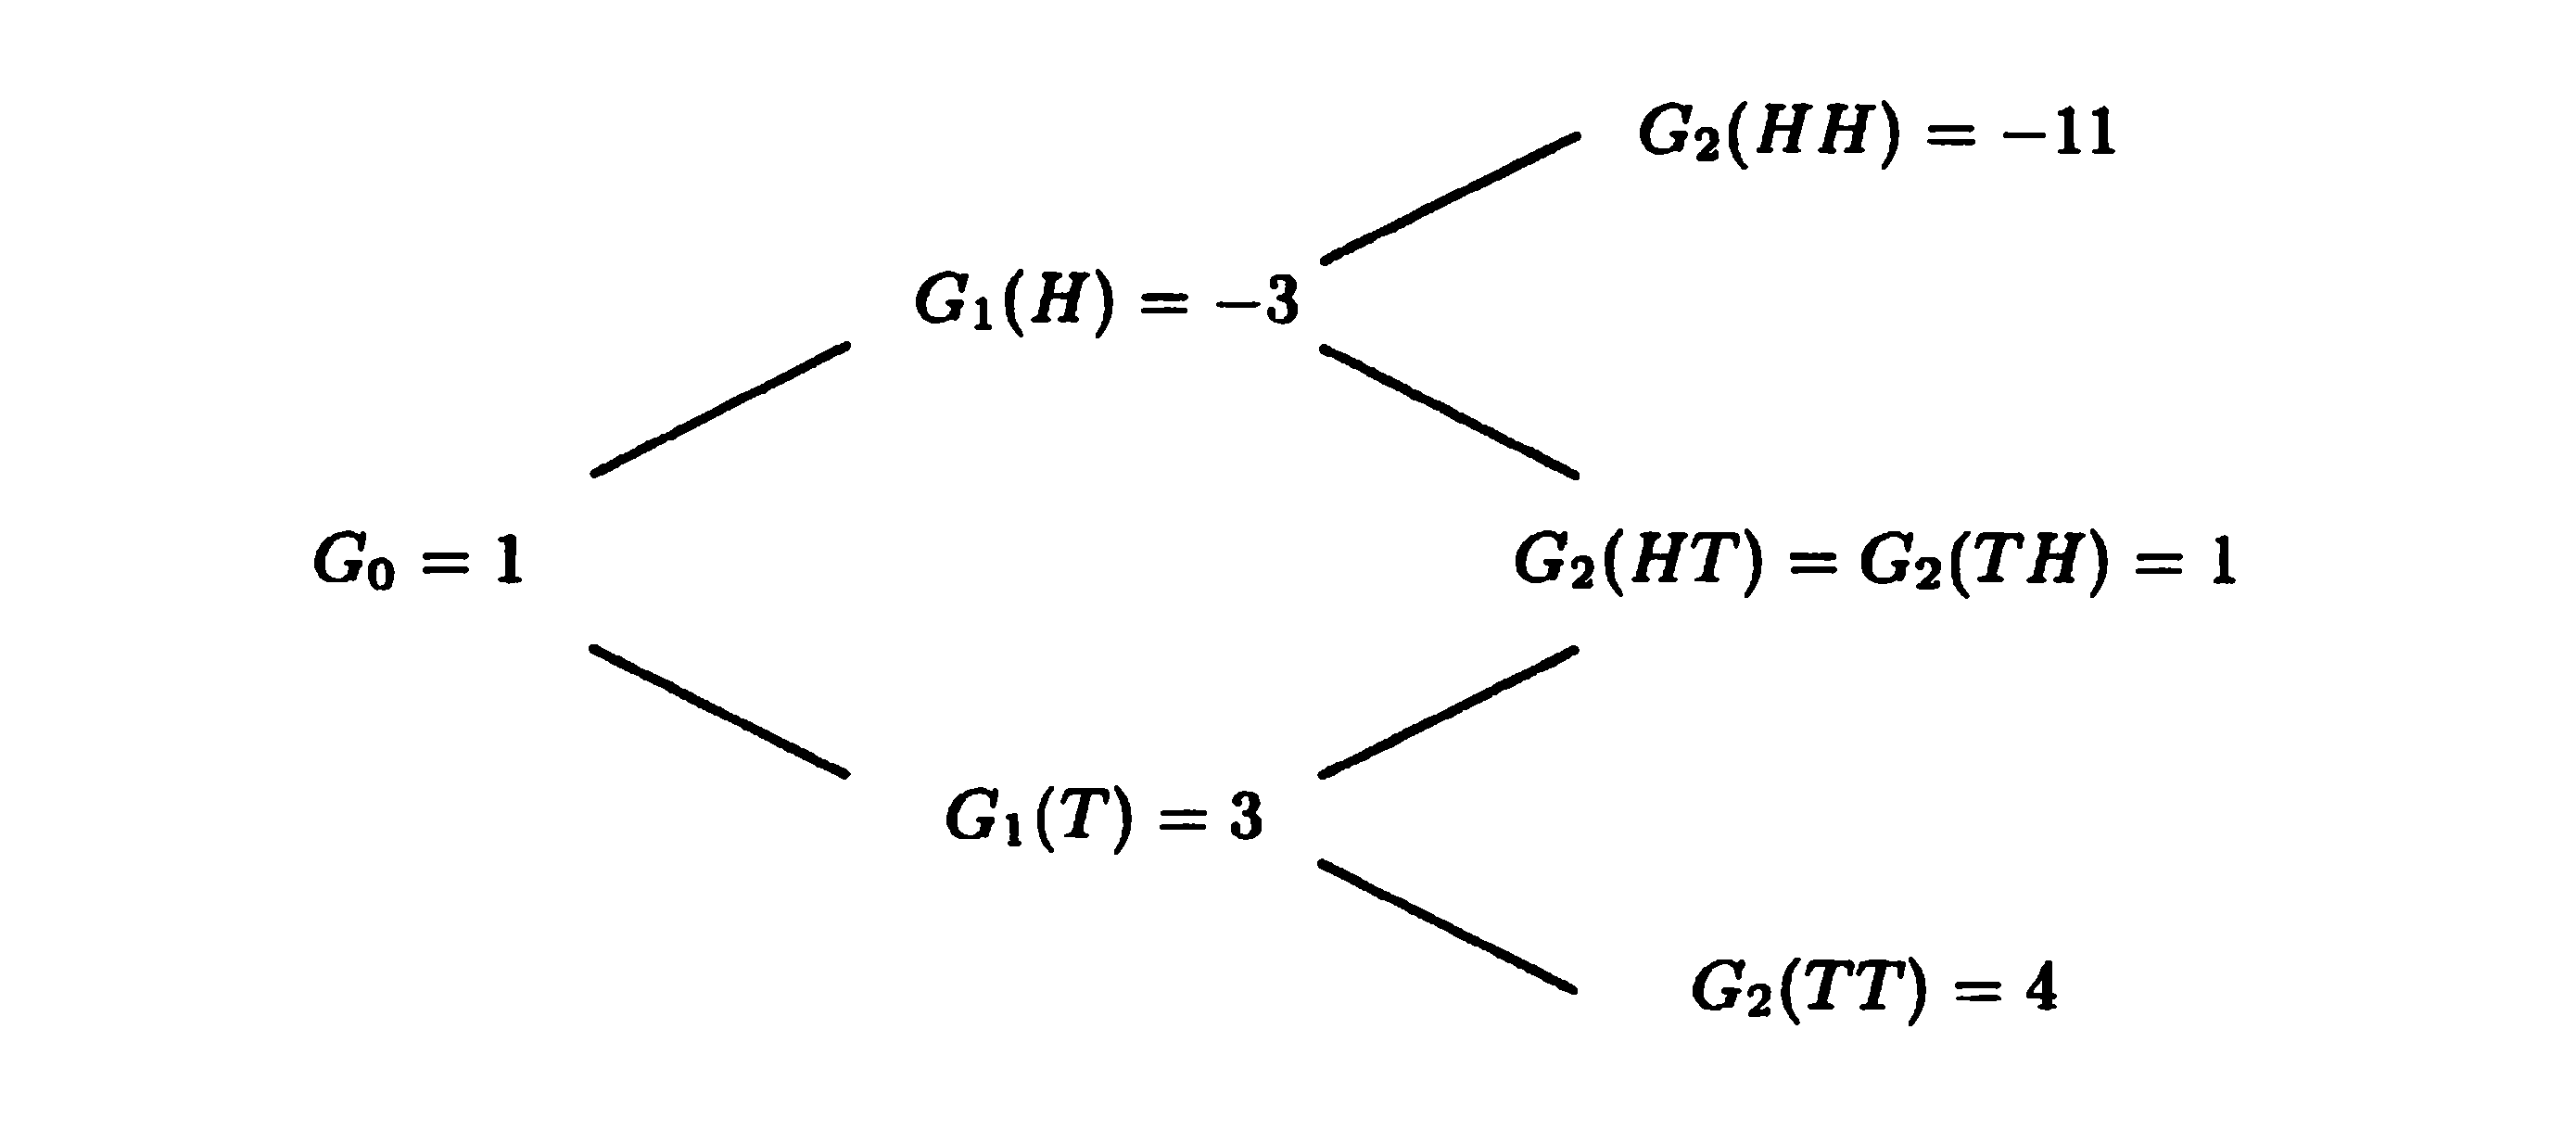
\includegraphics[width=0.9\linewidth]{screenshot005}
	\caption{Intrinsic value}
	\label{fig:screenshot005}
\end{figure}


\end{frame}




\begin{frame}[shrink=5]

\frametitle{\insertsection} 
\framesubtitle{\insertsubsection} 

\

We apply

\begin{equation}\label{e1}
V_n = \max_{\tau \in S_n} \tilde{E}_n [\mathbb{I}_{\{\tau \leq N\}} \dfrac{1}{(1+r)^{\tau-n}}G_{\tau}]
\end{equation}


with $n=1$, first considering the case of $H$ on the first toss. Then 

\begin{equation}\label{key}
V_1(H)=\max\limits_{{\tau \in S_1}}\widetilde{\mathbb{E}}_1\left [ \mathbb{I}_{(\tau\leq 2)}\left ( \frac{4}{5} \right )^{\tau-1}G_\tau \right ](H).
\end{equation}

To make conditional expectation as much as possible, we should take $\tau(HH)=\infty$  (do not exercise) and take $\tau(HT)= 2$ (exercise at time one in case of HT).

\

With this exercise policy we get:


\begin{equation}\label{key}
V_1(H)= \frac{1}{2}\cdot 0 + \frac{1}{2} \cdot \left ( \frac{4}{5} \right )^{2-1}G_2(HT) = 0.4
\end{equation}

\end{frame}



\begin{frame}[shrink=5]

\frametitle{\insertsection} 
\framesubtitle{\insertsubsection} 

\

We apply

\begin{equation}\label{e1}
V_n = \max_{\tau \in S_n} \tilde{E}_n [\mathbb{I}_{\{\tau \leq N\}} \dfrac{1}{(1+r)^{\tau-n}}G_{\tau}]
\end{equation}


with $n=1$, first considering the case of $T$ on the first toss. Then 

\begin{equation}\label{key}
V_1(H)=\max\limits_{{\tau \in S_1}}\widetilde{\mathbb{E}}_1\left [ \mathbb{I}_{(\tau\leq 2)}\left ( \frac{4}{5} \right )^{\tau-1}G_\tau \right ](T).
\end{equation}

To make this conditional expectation as large as possible, knowing that the first toss results in tail, we must consider two possibilities: exercise at time one or at time two. If we take $\tau(TH)= \tau(TT)= 1$, then

\begin{equation}\label{key}
\widetilde{\mathbb{E}}_1\left [ \mathbb{I}_{(\tau\leq 2)} \left ( \frac{4}{5} \right )^{\tau-1}G_\tau  \right ](T) = G_1(T) = 3.
\end{equation}

If we take $\tau(TH)= \tau(TT)= 2$, then

\begin{equation}\label{key}
\widetilde{\mathbb{E}}_1\left [ \mathbb{I}_{(\tau\leq 2)} \left ( \frac{4}{5} \right )^{\tau-1}G_\tau  \right ](T) = \frac{4}{5}\left ( \frac{1}{2}\cdot 1 + \frac{1}{2}\cdot 4\right ) = 2.
\end{equation}

Hence, $V_1(T) = 3$.

\end{frame}




\begin{frame}[shrink=5]

\frametitle{\insertsection} 
\framesubtitle{\insertsubsection} 

\

Finally, when n=0, we have


\begin{equation}\label{e11}
V_0 = \max\limits_{{\tau \in S_0}}\widetilde{\mathbb{E}}\left [ \mathbb{I}_{(\tau\leq 2)} \left ( \frac{4}{5} \right )^{\tau}G_\tau  \right ].
\end{equation}

Stopping time that makes (\ref{e11}) as large as possible is $\tau(HH)= \infty, \tau(TH)= \tau(TT)= 1, \tau(HT)= 2 $. With this stopping time it becomes:

\begin{equation}\label{key}
V_0 = \frac{1}{4}\cdot 0 + \frac{1}{4}\cdot \left (\frac{4}{5}  \right )^{2}\cdot G_2(HT)+\frac{1}{2}\cdot \frac{4}{5}\cdot G_1(T) = \frac{1}{4}\cdot \frac{16}{25}\cdot 1 + \frac{1}{2}\cdot \frac{4}{5}\cdot 3 = 1.36
\end{equation}


\begin{figure}
	\centering
	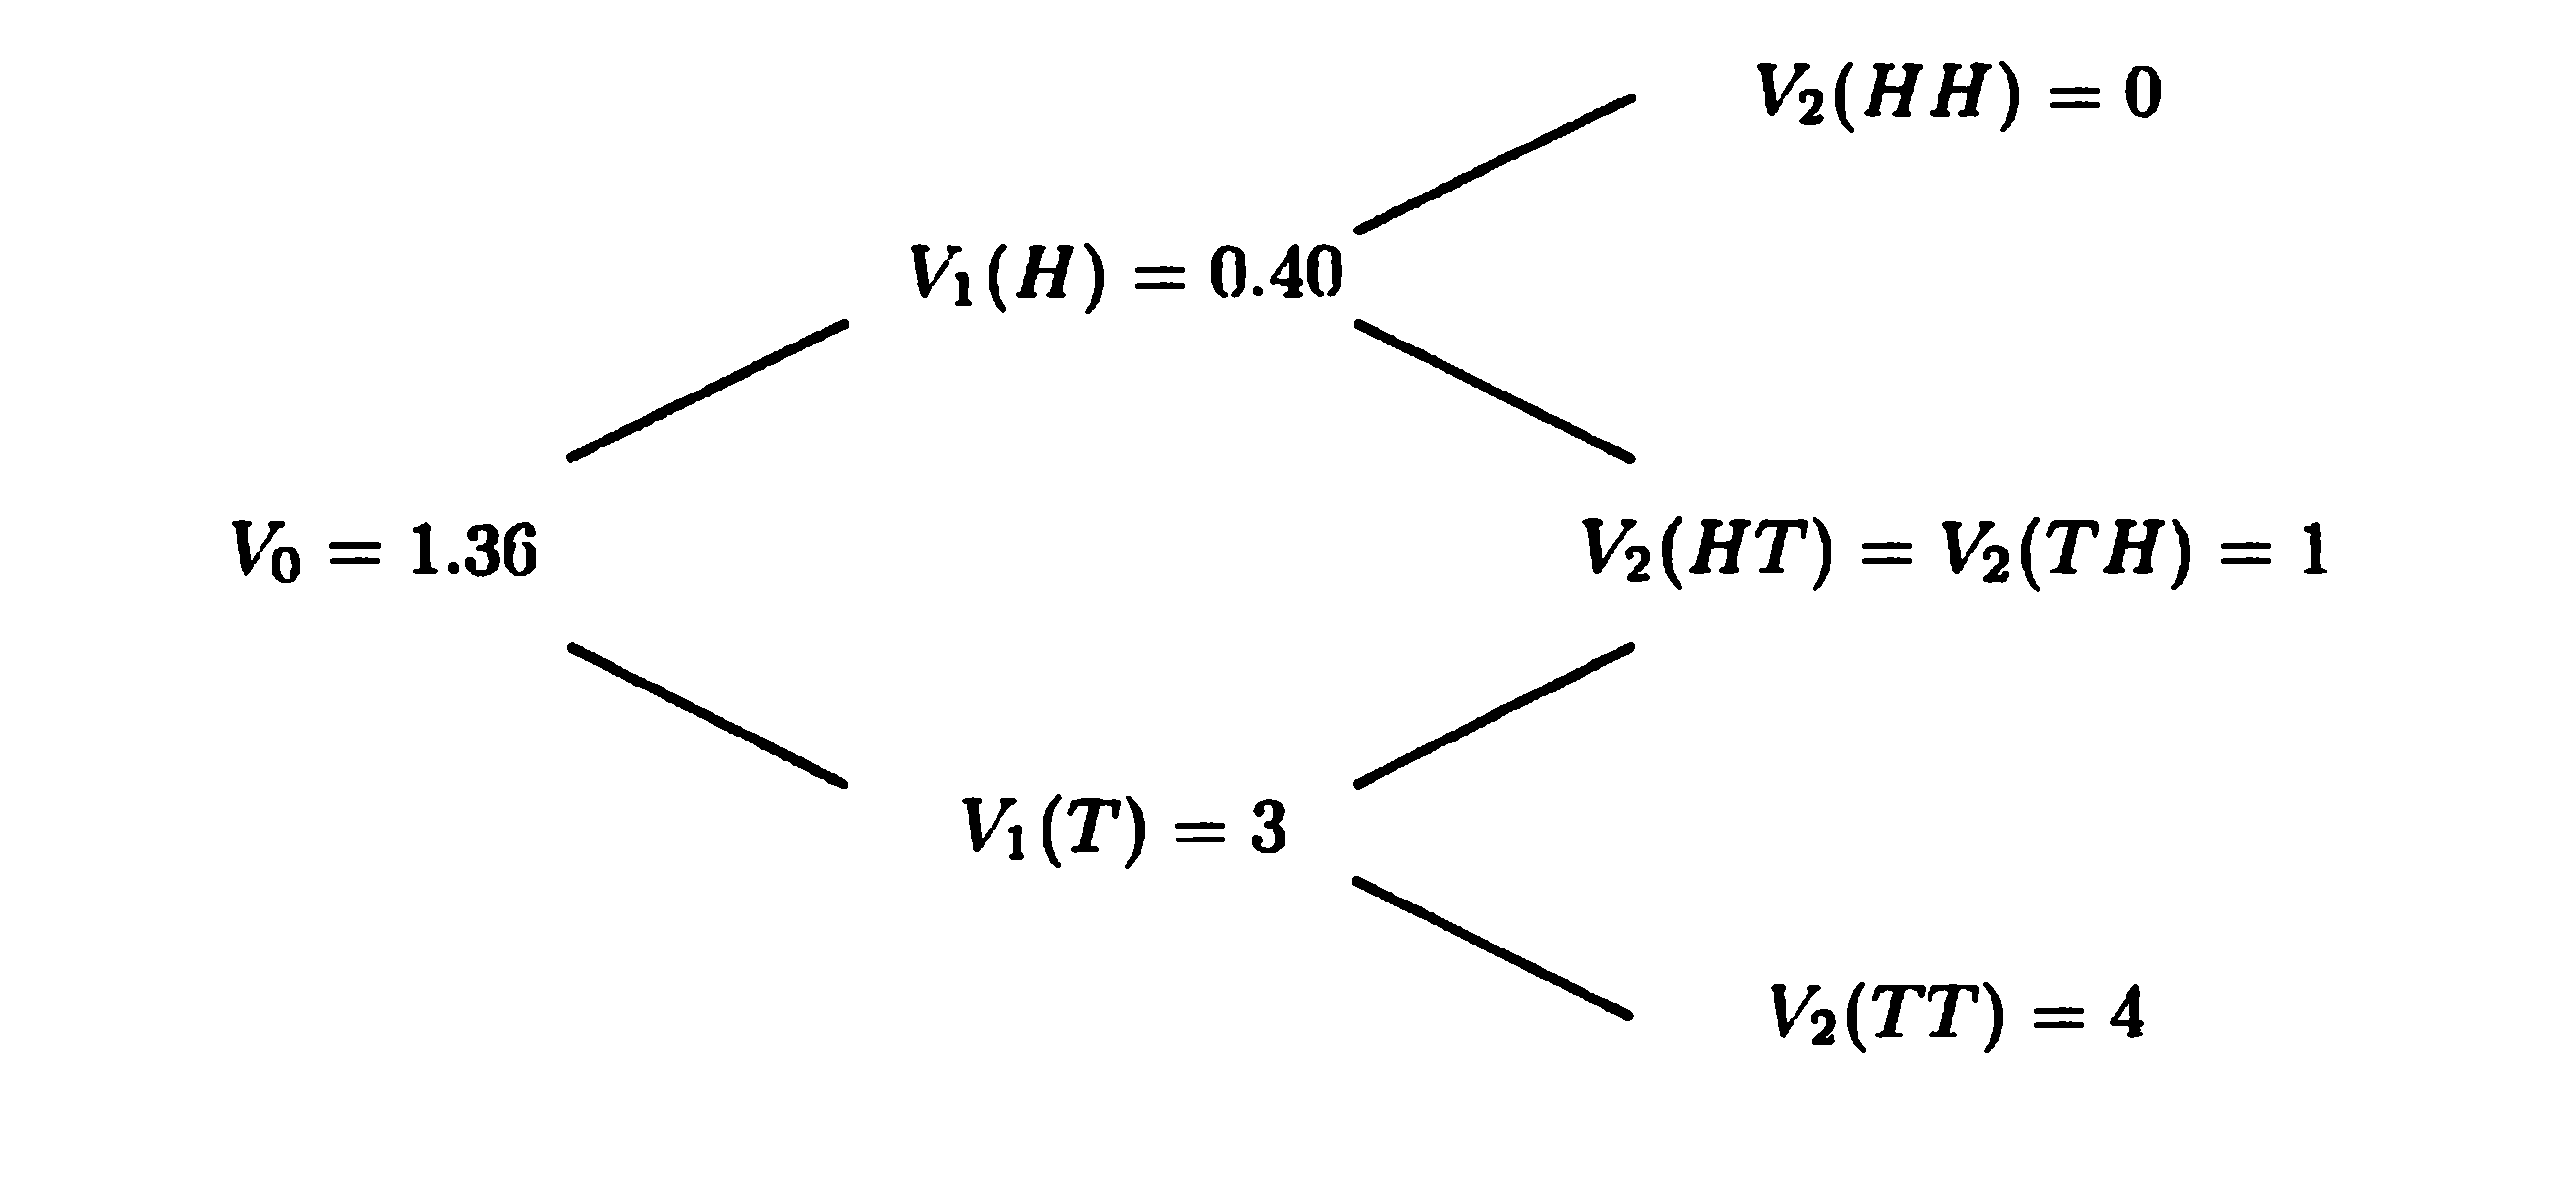
\includegraphics[width=0.7\linewidth]{screenshot007}
	\caption{American put prices}
	\label{fig:screenshot007}
\end{figure}


\end{frame}

\subsection{Properties}

\begin{frame}[shrink=5]

\frametitle{\insertsection} 
\framesubtitle{\insertsubsection} 


%\begin{frame}
%\frametitle{Theorem 4.4.2}
\begin{block}{Theorem 4.4.2}
	The American derivative security price process given by Definition 4.4.1 has the following properties:\\
	(i) $V_n\ge max\{G_n,0\}$ for all $n$;\\
	(ii) the discounted process $\frac{1}{(1+r)^n}V_n$ is a supermartingale;\\
	(iii) if $Y_n$ is another process satisfying $Y_n \ge max\{G_n,0\}$ for all $n$ and for which $\frac{1}{(1+r)^n}Y_n$ is a supermartingale. then $Y_n \ge V_n$ for all $n$.\\
	
	We summarize property (iii) by saying that $V_n$ is the smallest process satisfying (i) and (ii). 
\end{block}

We shall see that property (ii) in Theorem 4.4.2 guarantees that an agent beginning with initial capital $V_0$ can construct a hedging portfolio whose value at each time $n$ is $V_n$. Property (i) guarantees that if an agent does this, he has hedged a short position in the derivative security; no matter when it is exercised, the agent's hedging portfolio value is sufficient to pay off the derivative security. Thus, (i) and (ii) guarantee that the derivative security price is acceptable to the seller. Condition (iii) says that the price is no higher than necessary in order to be acceptable to the seller. This condition ensures that the price is fair for the buyer.

\end{frame}


\begin{frame}[shrink=5]

\subsection{Proof of theorem}

\frametitle{\insertsection} 
\framesubtitle{\insertsubsection} 

%
%\begin{frame}
%\frametitle{Proof of theorem}
We first establish (i). Let $n$ be given, and consider the stopping time $\widehat{\tau}$ in $\mathcal{S}_n$ that takes the value $n$, regardless of the coin tossing. Then
\begin{equation}\label{key}
\widetilde{\mathbb{E}}_n\left[\mathbb{I}_{\{\widehat{\tau}\le N\}}\frac{1}{(1+r)^{\widehat{\tau}-n}}G_{\tau}\right]=G_n.
\end{equation}
Since $V_n$ is the largest possible value we can obtain for $\widetilde{\mathbb{E}}_n\left[\mathbb{I}_{\{\tau\le N\}}\frac{1}{(1+r)^{\tau-n}}G_{\tau}\right]$ when we consider all stopping times $\tau\in \mathcal{S}_n$, we must have $V_n \ge G_n$. On the other hand, if we take $\overline{\tau}$ to be the stopping time in $\mathcal{S}_n$ that takes the value $\infty$, regardless of the coin tossing, then 
\begin{equation}\label{key}
\widetilde{\mathbb{E}}_n\left[\mathbb{I}_{\overline{\tau}\le N}\frac{1}{(1+r)^{\overline{\tau}-n}}G_{\overline{\tau}}\right]=0.
\end{equation}
Again, $V_n$ is the maximum of expressions of this type, and hence $V_n \ge 0$. We conclude that (i) holds.
\end{frame}

\begin{frame}[shrink=5]

\frametitle{\insertsection} 
\framesubtitle{\insertsubsection} 
%\begin{frame}
%\frametitle{Proof of theorem}
We next prove (ii). Let $n$ be given, and suppose $\tau^*$ attains the maximum 
in the definition of $V_{n+1}$; i.e., $\tau^*\in\mathcal{S}_n$ and
$$V_{n+1}=\widetilde{\mathbb{E}}_{n+1}\left[\mathbb{I}_{\{\tau^*\le N\}}\frac{1}{(1+r)^{\tau^*-n-1}}G_{\tau^*}\right]. \ \ \ \ \ \  (4.4.8)$$
But $\tau^*\in\mathcal{S}_n$ also, which together with iterated conditioning implies
$$V_{n}\ge\widetilde{\mathbb{E}}_{n}\left[\mathbb{I}_{\{\tau^*\le N\}}\frac{1}{(1+r)^{\tau^*-n}}G_{\tau^*}\right]=\widetilde{\mathbb{E}}_{n}\left[\widetilde{\mathbb{E}}_{n+1}\left[\mathbb{I}_{\{\tau^*\le N\}}\frac{1}{(1+r)^{\tau^*-n}}G_{\tau^*}\right]\right]$$
$$=\widetilde{\mathbb{E}}_{n}\left[\frac{1}{1+r}\widetilde{\mathbb{E}}_{n+1}\left[\mathbb{I}_{\{\tau^*\le N\}}\frac{1}{(1+r)^{\tau^*-n-1}}G_{\tau^*}\right]\right]=\widetilde{\mathbb{E}}_{n}\left[\frac{1}{1+r}V_{n+1}\right]. \ \ \ \ (4.4.9)$$
Dividing both sides by $(1+r)^n$, we obtain the supermartingale property for the discounted price process:
\begin{equation}\label{key}
\frac{1}{(1+r)^n}V_n\ge \widetilde{\mathbb{E}}_{n}\left[\frac{1}{(1+r)^{n+1}}V_{n+1}\right].
\end{equation}\end{frame}

\begin{frame}[shrink=5]

\frametitle{\insertsection} 
\framesubtitle{\insertsubsection} 
%\begin{frame}
%\frametitle{Proof of theorem}
Finally, we prove (iii). Let $Y_n$ be another process satisfying conditions (i) and (ii). Let $n \le N$ be given and let $\tau$ be a stopping time in $\mathcal{S}_n$. Because $Y_k \ge \max\{G_k,0\}$ for all $k$, we have
$$\mathbb{I}_{\{\tau\le N\}}G_{\tau}\le\mathbb{I}_{\{\tau\le N\}}\max\{G_{\tau},0\}\le\mathbb{I}_{\{\tau\le N\}}\max\{G_{N\wedge\tau},0\}+\mathbb{I}_{\{\tau=\infty\}}\max\{G_{N\wedge\tau},0\}$$
\begin{equation}\label{key}
=max\{G_{N\wedge\tau},0\}\le Y_{N\wedge\tau}.
\end{equation}
We next use the Optional Sampling Theorem 4.3.2 and the supermartingale property for $\frac{1}{(1+r)^k}Y_k$ to write
$$\widetilde{\mathbb{E}}_{n}\left[\mathbb{I}_{\tau\le N}\frac{1}{(1+r)^{\tau}}G_{\tau}\right]=\widetilde{\mathbb{E}}_{n}\left[\mathbb{I}_{\tau\le N}\frac{1}{(1+r)^{N\wedge\tau}}G_{\tau}\right]\le\widetilde{\mathbb{E}}_{n}\left[\frac{1}{(1+r)^{N\wedge\tau}}Y_{N\wedge\tau}\right]$$
\begin{equation}\label{key}
\le\frac{1}{(1+r)^{n\wedge\tau}}Y_{n\wedge\tau}=\frac{1}{(1+r)^{n}}Y_{n}
\end{equation}

the equality at the end being a consequence of the fact that $\tau\in\mathcal{S}_n$ is greater than or equal to $n$ on every path. Multiplying by $(1+r)^n$, we obtain
\begin{equation}\label{key}
\widetilde{\mathbb{E}}_{n}\left[\mathbb{I}_{\tau\le N}\frac{1}{(1+r)^{\tau-n}}G_{\tau}\right]\le Y_n.
\end{equation}
Since $V_n$ is the maximum value we can obtain for $\widetilde{\mathbb{E}}_{n}\left[\mathbb{I}_{\tau\le N}\frac{1}{(1+r)^{\tau-n}}G_{\tau}\right]$ as $\tau$ ranges over $\mathcal{S}_n$, and all these values are less than or equal to $Y_n$, we must 
have $V_n \le Y_n$. 

\end{frame}


\subsection{Algorithm for path-dependent derivative security price}

\begin{frame}[shrink=5]

\frametitle{\insertsection} 
\framesubtitle{\insertsubsection} 

%\begin{frame}
%\frametitle
\begin{block}{Theorem 4.4.3}
We have the following American pricing algorithm for the path-dependent derivative security price process given by Definition 4.4.1:
$$V_N(\omega_1...\omega_N)=\max\{G_N(\omega_1...\omega_N),0\} \ \ \ \ \ \ (4.4.10)$$
$$V_n(\omega_1...\omega_n)=\max\{G_n(\omega_1...\omega_n), \frac{1}{1+r}\left[\tilde{p}V_{n+1}(\omega_1...\omega_nH)+\tilde{q}V_{n+1}(\omega_1...\omega_nT)\right]\} \ \ \ (4.4.11)$$
for $n=N-1,...,0$.
\end{block}

We shall prove that $V_n$ defined recursively by (4.4.10) and (4.4.11) satisfies properties (i) and (ii) of Theorem 4.4.2 and is the smallest process with these properties. According to Theorem 4.4.2, the process $V_n$ given by (4.4.1) is the smallest process with these properties, and hence the algorithm (4.4.10), (4.4.11) must generate the same process as formula (4.4.1).\\

\

We first establish property (i) of Theorem 4.4.2. It is clear that $V_N$ defined by (4.4.10) satisfies property (i) with $n = N$. We proceed by induction 
backward in time. Suppose that for some $n$ between $0$ and $N-1$ we have $V_{n+1}\ge max\{G_{n+1},0\}$. Then, from (4.4.11), we see that
\begin{equation}\label{key}
V_n(\omega_1...\omega_n)\ge \max\{G_n(\omega_1...\omega_n),0\}.
\end{equation}
This completes the induction step and shows that $V_n$ defined recursively by (4.4.10), (4.4.11) satisfies property (i) of Theorem 4.4.2.
 
\end{frame}

\subsection{Proof of theorem}

\begin{frame}[shrink=5]

\frametitle{\insertsection} 
\framesubtitle{\insertsubsection} 

\

%\begin{frame}
%\frametitle{Proof of theorem}
We next verify that $\frac{1}{(1+r)^n}V_n$ is a supermartingale. From (4.4.11), we see immediately that 
\begin{equation}\label{key}
V_n(\omega_1...\omega_n)\ge \frac{1}{1+r}\left[\tilde{p}V_{n+1}(\omega_1...\omega_nH)+\tilde{q}V_{n+1}(\omega_1...\omega_nT)\right] =\widetilde{\mathbb{E}}_{n}\left[\frac{1}{1+r}V_{n+1}\right](\omega_1...\omega_n)\end{equation}

Multiplying both sides by $\frac{1}{(1+r)^n}$ we obtain the desired supermartingale property.\\

\

Finally, we must show that $V_n$ defined by (4.4.10), (4.4.11) and satisfying (i) and (ii) of Theorem 4.4.2 is the smallest process satisfying (i) and (ii). It is immediately clear from (4.4.10) that $V_N$ is the smallest random variable satisfying $V_N \ge \max\{G_N,0\}$. We proceed by induction backward in time. Suppose that, for some $n$ between $0$ and $N-1, V_{n+1}$ is as small as possible.

\

%\begin{frame}
%\frametitle{Proof of theorem}
The supermartingale property (ii) implies that $V_n$ must satisfy (4.4.12). In order to satisfy property (i), $V_n$ must be greater than or equal to $G_n$. Therefore, properties (i) and (ii) of Theorem 4.4.2 imply
\begin{equation*}\label{key}
V_n(\omega_1...\omega_n)=\max\{G_n(\omega_1...\omega_n),
\frac{1}{1+r}\left[\tilde{p}V_{n+1}(\omega_1...\omega_nH)+\tilde{q}V_{n+1}(\omega_1...\omega_nT)\right]\} \ \ \ \ \ \  \ \ \ \ (4.4.13)
\end{equation*}
for $n=N-1,...,0$. But (4.4.11) defines $V_n(\omega_1...\omega_n)$ to be equal to the right-hand side of (4.4.13), which means $V_n(\omega_1...\omega_n)$ is as small as possible. 

\end{frame}





\subsection{Replication of path-dependent American derivatives}



	
\begin{frame}[shrink=5]

\frametitle{\insertsection} 
\framesubtitle{\insertsubsection} 

Consider an N-period binomial asset-pricing model with no-arbitrage rule $0 < d < 1 + r < u$ and with risk-neutral probabilities

\begin{equation}\label{key}
\tilde{p}= \dfrac{1+r-d}{u-d}, \tilde{q}= \dfrac{u-1-r}{u-d}.
\end{equation}
Let $G_n$ be a random variable depending on the first n coin tosses. An American derivative security with intrinsic value process $G_n$ is a contract that can be exercised at any time prior to and including time $N$ and, if exercised at time $n$, pays off $G_n$ with the price process $V_n$:

\begin{equation}\label{eq1}
V_n = \max_{\tau \in S_n} \tilde{E}_n [\mathbb{I}_{\{\tau \leq N\}} \dfrac{1}{(1+r)^{\tau-n}}G_{\tau}].
\end{equation}

In order to justify the definition for American derivative security prices,
we must show that a short$^{1}$ position can be hedged using these prices. 

\

This requires a generalization of Theorem 4.2.2 (Replication of path-independent derivative) to the path-dependent case.

\

\

\


\

\

\
\footnotesize{$^{1}$ A short, or a short position, is created when a trader sells a security first with the intention of repurchasing it or covering it later at a lower price. } 

\end{frame}



\begin{frame}[shrink=5]
\frametitle{\insertsection} 
\framesubtitle{\insertsubsection} 

Let

\begin{equation}\label{key}
\Delta_n(w_1...w_n) = \dfrac{V_{n+1}(w_1...w_nH) -V_{n+1}(w_1...w_nT)   }{S_{n+1}(w_1...w_nH) -S_{n+1}(w_1...w_nT) }
\end{equation}
\begin{multline}\label{key}
C_n(w_1...w_n) = V_n(w_1...w_n) - \dfrac{1}{1+r  } [\tilde{p}V_{n+1}(w_1...w_nH)  + \tilde{q}V_{n+1}(w_1...w_nT) ]
\end{multline}
where  $S_n$ -- the stock price at time $n$, $w_n\in \{H,T\}$ -- result of a coin toss at time $n$. 


%123

\begin{block}{Theorem 4.4.4}
\begin{enumerate}
	\item 
 We have $C_n>0, \forall n$.


\item  If we set $X_0 = V_0$ and define recursively forward in time the portfolio values $X_1, X_2,..., X_N$ by

\begin{equation}\label{key}
X_{n+1} = \Delta_n S_{n+1} + (1+r)(X_n-C_n-\Delta_nS_n)
\end{equation}

then we have

\begin{equation}\label{key}
X_n(w_1...w_n) = V_n(w_1...w_n), \forall n, \forall w_1...w_n.
\end{equation}

\item  In particular $X_n > G_n, \forall n.$
\end{enumerate}
\end{block}
	
\end{frame}
	
	
\begin{frame}[shrink=5]
\frametitle{\insertsection} 
\framesubtitle{\insertsubsection} 



\begin{block}{Proof 4.4.4}
\end{block}

\begin{enumerate}
	\item  The nonnegativity of $C_n$ is a consequence of the fact that the discounted process $\dfrac{1}{(1+r)^n}V_n$ is a supermartingale.

 The induction hypothesis is that  $X_n(w_1...w_n) = V_n(w_1...w_n)$ for some $n \in \{0, ..., N-1\},   \forall w_1...w_n. $ We fix $w_1...w_n$  for the rest of the proof, so by definition: 


\begin{equation}\label{key}
V_n - C_n = \dfrac{1}{1+r  } [\tilde{p}V_{n+1}(H)  + \tilde{q}V_{n+1}(T) ]
\end{equation}



\item \begin{multline}
X_{n+1}(H) = \Delta_n S_{n+1}(H) + (1+r) (X_n-C_n-\Delta_n S_{n}) =  \dfrac{V_{n+1}(H) -V_{n+1}(T)   }{S_{n+1}(H) -S_{n+1}(T) } \\  (Sn+1(H)-(1+r)S_n)+(1+r)(V_n-C_n)= \dfrac{V_{n+1}(H) -V_{n+1}(T)   }{(u-d)S_{n} } (uS_n-(1+r)S_n)+ \\ + \tilde{p}V_{n+1}(H) +\tilde{q}V_{n+1}(T) = (V_{n+1}(H)-V_{n+1}(T)) \dfrac{u-1-r}{u-d} + \tilde{p}V_{n+1}(H) +\tilde{q}V_{n+1}(T) = \\ = (V_{n+1}(H)-V_{n+1}(T)) \tilde{q} + \tilde{p}V_{n+1}(H) +\tilde{q}V_{n+1}(T) = (\tilde{q} + \tilde{p})  V_{n+1}(H) =  V_{n+1}(H)
 \end{multline}

The proof of  $X_n(w_1...w_nT) = V_n(w_1...w_nT)$ is  analogous.

\

\item The fact that  $X_n > G_n, \forall n$  follows from $X_n(w_1...w_n) = V_n(w_1...w_n), \forall n, \forall w_1...w_n$  and
$V_n \geq \max{G_n,0} , \forall n$

\end{enumerate}

\end{frame}	


\begin{frame}[shrink=5]
\frametitle{\insertsection} 
\framesubtitle{\insertsubsection} 

			Theorem 4.4.4 shows that the American derivative security price given by (\ref{eq1}) is acceptable to the seller because he can construct a hedge for the
			short position. 			We next argue that it is also acceptable to the buyer. 
			
			\
			
			Let us 		fix $n$, imagine we have gotten to time $n$ without the derivative security being exercised, and denote by $\tau^* \in S_n$  the stopping time that attains the maximum price: 
			
			\begin{equation}\label{eq2}
			V_n =  \tilde{E}_n [\mathbb{I}_{\{\tau^* \leq N\}} \dfrac{1}{(1+r)^{\tau^*-n}}G_{\tau}].
			\end{equation}
			
			
			If the owner of the derivative security exercises it according to the stopping 
			time $\tau*$, then he will receive the cash flows $C_n, C_{n+i},..., C_N$, where

\begin{equation}\label{key}
C_k = \mathbb{I}_{\{\tau*=k\}G_k},  k = n,n+1,...,N
\end{equation}


			 Actually, at most one of these $C_k$  values is non-zero.
			If the option is exercised at or before the expiration time $N$, then the $C_k$
			corresponding to the exercise time is the only nonzero payment among them. However, on different paths, this payment comes at different times. 
			
			In any
			case, (\ref{eq2}) becomes the net present value at time $n$  of
			the cash flows:
			
			
				
			\begin{equation}\label{eq2}
			V_n =  \tilde{E}_n \left[\sum^N_{k=n}\mathbb{I}_{\{\tau^* =k\}} \dfrac{1}{(1+r)^{k-n}}G_k \right] = \tilde{E}_n \left[\sum^N_{k=n} \dfrac{C_k}{(1+r)^{k-n}}\right].
			\end{equation}
			
%			59
%			p 125
			
			
			
			Once the option holder decides on the exercise strategy $\tau*$, this is exactly
			the contract she holds. Thus, the American derivative security price $V_n$ is
			acceptable to him.
			



\end{frame}	

\subsection{Optimal exercise}

\begin{frame}[shrink=5]
\frametitle{\insertsection} 
\framesubtitle{\insertsubsection} 

It remains to provide a method for the American derivative security owner
to choose an optimal exercise time. We shall consider this problem with $n = 0$ 
(i.e., seek a stopping time $\tau* \in S_0$  that achieves the maximum price  when
n = 0).

\begin{block}{Theorem 4.4.5}


The stopping time $\tau^*=min\{n;V_n = G_n\} $  maximizes the right-hand side of 

\begin{equation}\label{eq1}
V_n = \max_{\tau \in S_n} \tilde{E}_n [\mathbb{I}_{\{\tau \leq N\}} \dfrac{1}{(1+r)^{\tau-n}}G_{\tau}].
\end{equation}

when $n=0$; i.e.,

\begin{equation}\label{eq1}
V_0 =  \tilde{E} [\mathbb{I}_{\{\tau^* \leq N\}} \dfrac{1}{(1+r)^{\tau^*}}G_{\tau^*}].
\end{equation}

	
\end{block}

The value of an American derivative security is always greater than or
equal to its intrinsic value. The stopping time $\tau^*$  is the first time
these two are equal. 

\

It may be that they are never equal. For example, the
value of an American put is always greater than or equal to zero, but the put
can always be out of the money (i.e., with negative intrinsic value). In this
case, the minimum is taken over the empty set (the set of integers $n$ for
which $V_n = G_n$ is the empty set), and we follow the mathematical convention
that the minimum over the empty set is $\infty$. 

\

For us, $\tau^* = \infty$ is synonymous
with the derivative security expiring unexercised.


\end{frame}	

\begin{frame}[shrink=5]
\frametitle{\insertsection} 
\framesubtitle{\insertsubsection} 


\begin{block}{Proof 4.4.5}
\end{block}

 We first observe that the stopped process

\begin{equation}\label{k33}
\dfrac{1}{(1+r)^{n \wedge \tau^*} } V_{n \wedge \tau^*}
\end{equation}

is a martingale under the risk-neutral probability measure. This is a consequence of theorem about algorithm for the path dependent derivative security price process.  

\


Indeed, if the first $n$ coin tosses result in $w_1...w_n$ (fixed from here) and
along this path $\tau^* \geq n + 1$, then we know that $V_n > G_n$  and by  Theorem 4.4.3:

\begin{multline}
V_{n \wedge \tau^*} = V_n = \dfrac{1}{1+r} [\tilde{p}V_{n+1}(H)  + \tilde{q}V_{n+1}(T) ] = \dfrac{1}{1+r} [\tilde{p}V_{(n+1) \wedge \tau^*}(H)  + \tilde{q}V_{(n+1) \wedge \tau^*}(T) ].
\end{multline}
This is the martingale property for the process (\ref{k33}). 

\end{frame}	



\begin{frame}[shrink=5]
\frametitle{\insertsection} 
\framesubtitle{\insertsubsection} 


\begin{block}{Proof 4.4.5 (continued)}
\end{block}

On the other hand,
if along the path  $w_1...w_n$ we have $\tau^* < n$, then


\begin{equation}
V_{n \wedge \tau^*} = V_\tau^* = \tilde{p}V_{\tau^*}  + \tilde{q}V_{\tau^*}  = \tilde{p}V_{(n+1) \wedge \tau^*}(H)  + \tilde{q}V_{(n+1) \wedge \tau^*}(T) ].
\end{equation}

Again we have the martingale property.

Since the stopped process (\ref{k33}) is a martingale, we have

\begin{multline}
V_0  = \tilde{E} \left[ \dfrac{1}{(1+r)^{N \wedge \tau^*} } V_{N \wedge \tau^*}  \right] = \tilde{E} \left[ \mathbb{I}_{\{\tau^* < N\}} \dfrac{1}{(1+r)^{ \tau^*} } G_{\tau^*}  \right]  + \tilde{E} \left[ \mathbb{I}_{\{\tau^* = \infty\}} \dfrac{1}{(1+r)^{N } } V_{N }  \right].
\end{multline}

But on those paths for which $\tau^* = \infty$, we must have $V_n > G_n, \forall n $  and,
in particular, $V_N > G_N$. 

Knowing the fact that 

\begin{equation}\label{key}
V_N(\omega_1...\omega_N)=max\{G_N(\omega_1...\omega_N),0\}
\end{equation}

this can only happen if $G_N < 0$
and $V_N = 0$. Therefore, $\mathbb{I}_{\{\tau^* = \infty\}}V_N=0$  and 

\begin{equation}
V_0  = \tilde{E} \left[ \mathbb{I}_{\{\tau^* < N\}} \dfrac{1}{(1+r)^{ \tau^*} } G_{\tau^*}  \right]  .
\end{equation}



\end{frame}	

\section{American Call Option}
\subsection{Introduction}

\begin{frame}[shrink=5]
\frametitle{\insertsection} 
\framesubtitle{\insertsubsection} 

Call option, often simply labeled a "call", is a contract, between the buyer and the seller of the call option, to exchange a security at a set price.

\

We can depict the payoff (to the buyer) of a call option upon expiration:


\begin{figure}
	\centering
	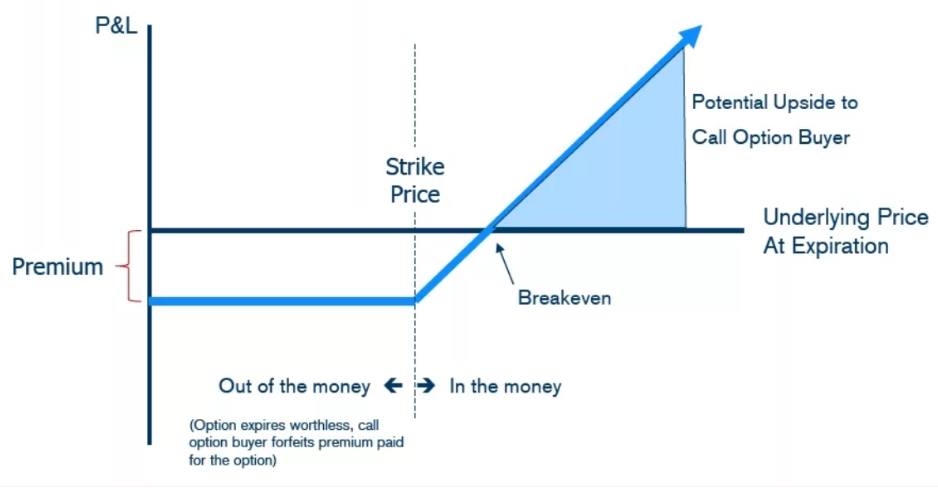
\includegraphics[width=0.9\linewidth]{screenshot001}
	\caption[Call option payoff diagram]{Call option payoff diagram}
	\label{fig:screenshot001}
\end{figure}


Financial risk is limited by the amount of the premium paid. 



\end{frame}	

\begin{frame}[shrink=5]
\frametitle{\insertsection} 
\framesubtitle{\insertsubsection} 

\begin{figure}
	\centering
	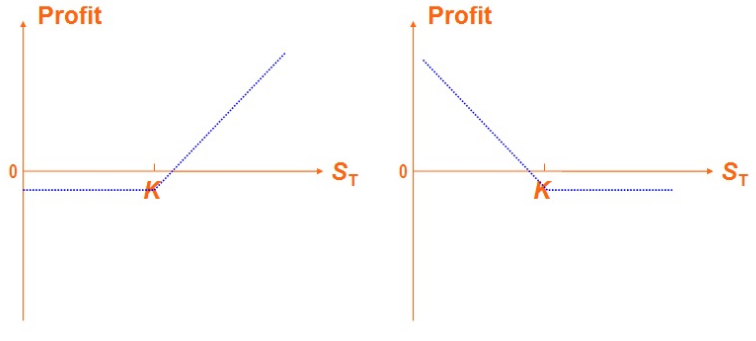
\includegraphics[width=0.6\linewidth]{screenshot003}
	\caption[Call option vs Put option]{Call option vs Put option}
	\label{fig:screenshot001}
\end{figure}

\begin{figure}
	\centering
	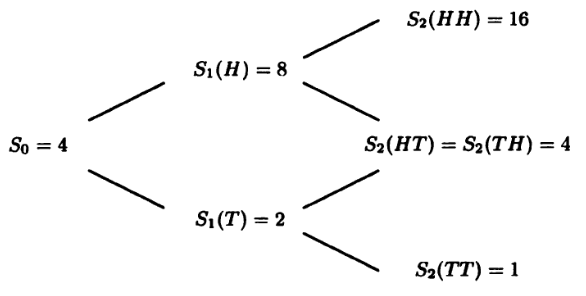
\includegraphics[width=0.4\linewidth]{screenshot002}
	\caption[A two period model]{A two period model}
	\label{fig:screenshot001}
\end{figure}


\end{frame}	

\subsection{Jensen's inequality }


\begin{frame}[shrink=5]
\frametitle{\insertsection} 
\framesubtitle{\insertsubsection} 

\

Let $g: [0, \infty) \to \mathbb{R}$

\begin{equation}\label{key}
g(\lambda s_1 + (1-\lambda) s_2) \leq   \lambda g( s_1)  + (1-\lambda) g(s_2), 
\end{equation}

\

where $ s_1 \geq 0, s_2 \geq 0$ and  $0\leq \lambda \leq 1$.


\begin{figure}
	\centering
	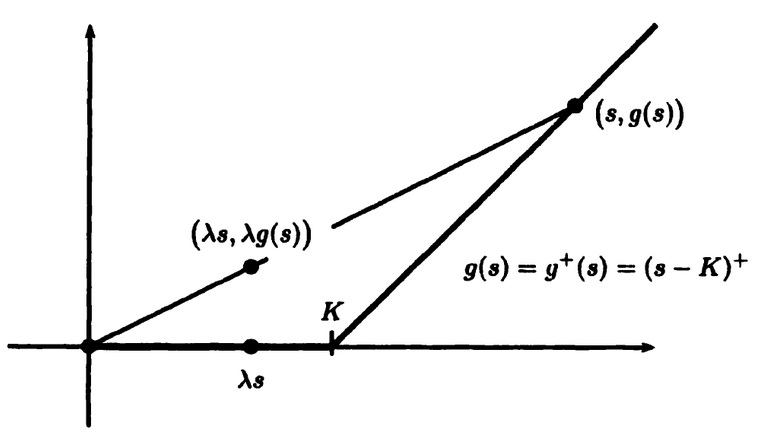
\includegraphics[width=0.8\linewidth]{screenshot004}
	\caption{Convex function with $g(0) = 0 $}
	\label{fig:screenshot004}
\end{figure}



\end{frame}	

\subsection{Value of Call option}

\begin{frame}[shrink=5]
\frametitle{\insertsection} 
\framesubtitle{\insertsubsection} 

\begin{block}{Theorem 4.5.1}

Consider an American derivative
security with convex payoff function $g(s)$ satisfying $g(0) = 0$. The value of this  derivative security at time zero, which is:

\begin{equation}\label{q}
V_0^A = \max_{\tau \in S_0} \tilde{E}_n [\mathbb{I}_{\{\tau \leq N\}} \dfrac{1}{(1+r)^{\tau}} g(S_{\tau})]
\end{equation}

is the same as the value of the European derivative security with payoff $g(S_N)$ 	at expiration $N$, which is 

\begin{equation}\label{q}
V_0^E =  \tilde{E}_N \left[ \dfrac{1}{(1+r)^{\tau}} \max \{ g(S_{N}, 0 )\}\right].
\end{equation}


\end{block}

Theorem 4.5.1 shows that the early exercise feature of the American call
contributes nothing to its value, because the discounted intrinsic value of the call is a submartingale under the risk-neutral probabilities.

\

The discounted intrinsic value of an American put is not a submartingale. 
Because the owner of the put receives
$К$ upon exercise, he may exercise early in order to prevent the value of this
payment from being discounted away. For low stock prices early exercise becomes optimal. 

\

For the call, the owner pays $К$ and prefers that the value of this payment
be discounted away before exercise. This reinforces the convexity effect and
makes early exercise undesirable.



\end{frame}	
	
\end{document}	